\documentclass{standalone}
\usepackage{tikz, pgfplots}

\begin{document}
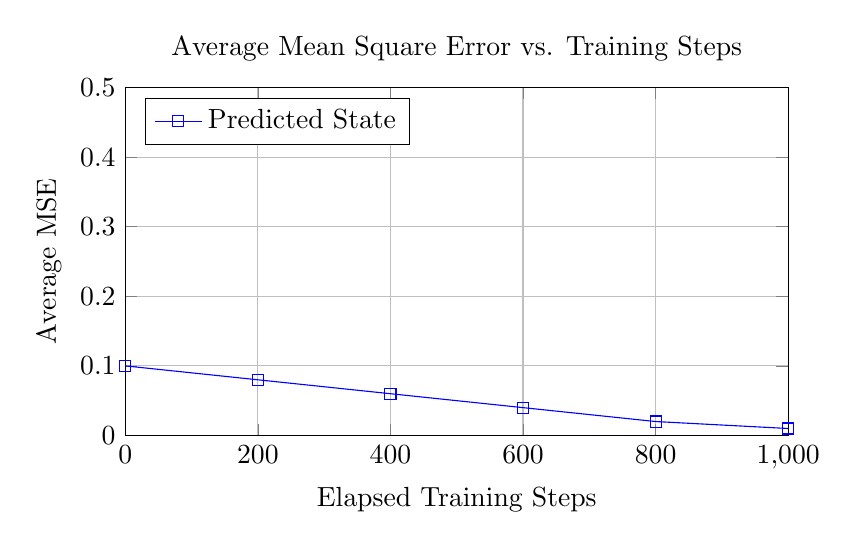
\begin{tikzpicture}
    \begin{axis}[
        title={Average Mean Square Error vs. Training Steps},
        xlabel={Elapsed Training Steps},
        ylabel={Average MSE},
        xmin=0,
        xmax=1000,
        ymin=0,
        ymax=0.5,
        grid=major,
        xtick distance=200,
        ytick distance=0.1,
        legend pos=north west,
        width=10cm,
        height=6cm
    ]
        % Example data points
        \addplot[blue, mark=square] coordinates {
            (0, 0.1)
            (200, 0.08)
            (400, 0.06)
            (600, 0.04)
            (800, 0.02)
            (1000, 0.01)
        };
        \legend{Predicted State}
    \end{axis}
\end{tikzpicture}
\end{document}